\documentclass{article}
\usepackage{tikz}
\usepackage{pgfplots}
\pgfplotsset{compat=1.8}

\newcommand{\colorone}{blue}
\newcommand{\colortwo}{red}

\begin{document}

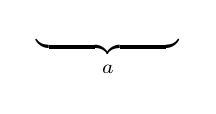
\begin{tikzpicture}
 \draw (-1,-.25) node {$\underbrace{\makebox[1.8cm]{}}_a$};
\end{tikzpicture}

\marginpar{%
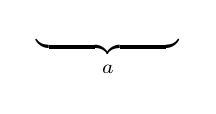
\begin{tikzpicture}
 \draw (-1,-.25) node {$\underbrace{\makebox[1.8cm]{}}_a$};
\end{tikzpicture}%
}

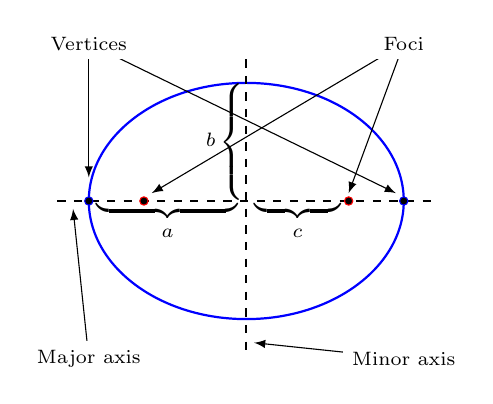
\begin{tikzpicture}
 \draw [thick,draw={\colorone}] (0,0) circle [x radius=2,y radius=1.5];
 \draw [thick,dashed] (-2.4,0) -- (2.4,0) (0,1.8) -- (0,-1.9);
 \filldraw [draw={\colortwo}] (1.3,0) circle (1.5pt) (-1.3,0) circle (1.5pt);
 \draw [->,>=latex] (-2,-2) node [fill=white] {\scriptsize Major axis}
  -- (-2.2,-.1);
 \draw [->,>=latex] (2,-2) node [fill=white] {\scriptsize Minor axis}
  -- (.1,-1.8);
 \draw [->,>=latex] (-2,2)  -- (-2,.3);
 \draw [->,>=latex] (-2,2) node [fill=white] {\scriptsize Vertices} -- (1.9,.1);
 \draw [->,>=latex] (2,2)  -- (-1.2,.1);
 \draw [->,>=latex] (2,2) node [fill=white] {\scriptsize Foci} -- (1.3,.1);
 \filldraw [draw={\colorone}] (2,0) circle (1.5pt) (-2,0) circle (1.5pt);
 \draw (-1,-.25) node {$\underbrace{\makebox[1.8cm]{}}_a$};
 \draw (.65,-.25) node {$\underbrace{\makebox[1.1cm]{}}_c$};
 \draw (-.25,.75) node [] {\scriptsize $b\left\{\rule[-.65cm]{0pt}{1.3cm}\right.$};
\end{tikzpicture}

\marginpar{%
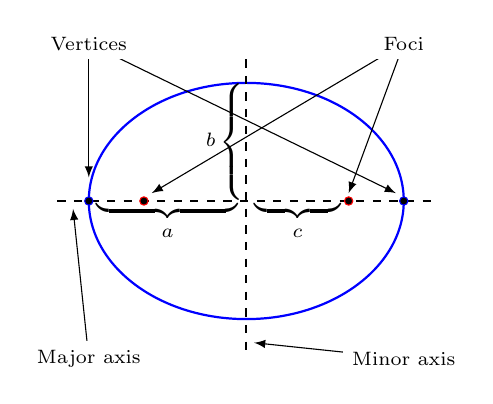
\begin{tikzpicture}
 \draw [thick,draw={\colorone}] (0,0) circle [x radius=2,y radius=1.5];
 \draw [thick,dashed] (-2.4,0) -- (2.4,0) (0,1.8) -- (0,-1.9);
 \filldraw [draw={\colortwo}] (1.3,0) circle (1.5pt) (-1.3,0) circle (1.5pt);
 \draw [->,>=latex] (-2,-2) node [fill=white] {\scriptsize Major axis}
  -- (-2.2,-.1);
 \draw [->,>=latex] (2,-2) node [fill=white] {\scriptsize Minor axis}
  -- (.1,-1.8);
 \draw [->,>=latex] (-2,2)  -- (-2,.3);
 \draw [->,>=latex] (-2,2) node [fill=white] {\scriptsize Vertices} -- (1.9,.1);
 \draw [->,>=latex] (2,2)  -- (-1.2,.1);
 \draw [->,>=latex] (2,2) node [fill=white] {\scriptsize Foci} -- (1.3,.1);
 \filldraw [draw={\colorone}] (2,0) circle (1.5pt) (-2,0) circle (1.5pt);
 \draw (-1,-.25) node {$\underbrace{\makebox[1.8cm]{}}_a$};
 \draw (.65,-.25) node {$\underbrace{\makebox[1.1cm]{}}_c$};
 \draw (-.25,.75) node [] {\scriptsize $b\left\{\rule[-.65cm]{0pt}{1.3cm}\right.$};
\end{tikzpicture}%
}

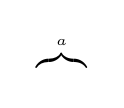
\begin{tikzpicture}
\draw (-.5,.4) node {\scriptsize $\overbrace{\makebox[18pt]{}}^a$};
\end{tikzpicture}

\marginpar{%
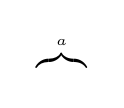
\begin{tikzpicture}
\draw (-.5,.4) node {\scriptsize $\overbrace{\makebox[18pt]{}}^a$};
\end{tikzpicture}%
}

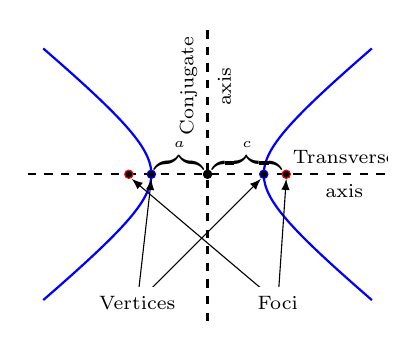
\begin{tikzpicture}
\begin{axis}[width=175pt,tick label style={font=\scriptsize},
axis y line=none,axis x line=none,name=myplot,
ymin=-3.2,ymax=3.2,xmin=-3.2,xmax=3.2]
\addplot [thick, draw={\colorone},smooth,domain=-70:70,samples=60] ({sec(x)},{tan(x)});
\addplot [thick, draw={\colorone},smooth,domain=-70:70,samples=60] ({-sec(x)},{tan(x)});
\filldraw (axis cs:0,0)  circle (1.5pt);
\draw [thick,dashed] 	(axis cs:-3.2,0)
 --  node [above,pos=.88] {\scriptsize Transverse}
 node [below,pos=.88] {\scriptsize axis}(axis cs:3.2,0)
 (axis cs:0,-3.2)
 -- node [below,rotate=90,pos=.8] {\scriptsize  axis }
 node [above,rotate=90,pos=.8] {\scriptsize Conjugate}(axis cs:0,3.2);
\filldraw [draw={\colorone}] (axis cs:1,0)circle(1.5pt) (axis cs:-1,0)circle(1.5pt);
\filldraw [draw={\colortwo}] (axis cs:1.4,0)circle(1.5pt) node (f1) {}
						(axis cs:-1.4,0)  circle (1.5pt) node (f2) {};
\draw [->,>=latex] (axis cs: 1.25,-2.8) -- (axis cs: -1.35,-.1);
\draw [->,>=latex] (axis cs: 1.25,-2.8) node [fill=white] {\scriptsize Foci }
 -- (axis cs: 1.4,-.1);	
\draw [->,>=latex] (axis cs: -1.25,-2.8) -- (axis cs: -1,-.1);
\draw [->,>=latex] (axis cs: -1.25,-2.8) node [fill=white] {\scriptsize Vertices}
 -- (axis cs: .95,-.1);	
\draw (axis cs:-.5,.4) node {\scriptsize $\overbrace{\makebox[18pt]{}}^a$};
\draw (axis cs:.7,.4) node {\scriptsize $\overbrace{\makebox[25pt]{}}^c$};
\end{axis}
\end{tikzpicture}

\marginpar{%
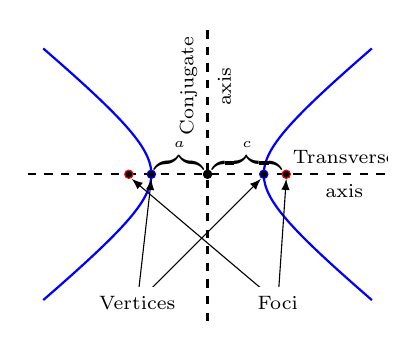
\begin{tikzpicture}
\begin{axis}[width=175pt,tick label style={font=\scriptsize},
axis y line=none,axis x line=none,name=myplot,
ymin=-3.2,ymax=3.2,xmin=-3.2,xmax=3.2]
\addplot [thick, draw={\colorone},smooth,domain=-70:70,samples=60] ({sec(x)},{tan(x)});
\addplot [thick, draw={\colorone},smooth,domain=-70:70,samples=60] ({-sec(x)},{tan(x)});
\filldraw (axis cs:0,0)  circle (1.5pt);
\draw [thick,dashed] 	(axis cs:-3.2,0)
 --  node [above,pos=.88] {\scriptsize Transverse}
 node [below,pos=.88] {\scriptsize axis}(axis cs:3.2,0)
 (axis cs:0,-3.2)
 -- node [below,rotate=90,pos=.8] {\scriptsize  axis }
 node [above,rotate=90,pos=.8] {\scriptsize Conjugate}(axis cs:0,3.2);
\filldraw [draw={\colorone}] (axis cs:1,0)circle(1.5pt) (axis cs:-1,0)circle(1.5pt);
\filldraw [draw={\colortwo}] (axis cs:1.4,0)circle(1.5pt) node (f1) {}
						(axis cs:-1.4,0)  circle (1.5pt) node (f2) {};
\draw [->,>=latex] (axis cs: 1.25,-2.8) -- (axis cs: -1.35,-.1);
\draw [->,>=latex] (axis cs: 1.25,-2.8) node [fill=white] {\scriptsize Foci }
 -- (axis cs: 1.4,-.1);	
\draw [->,>=latex] (axis cs: -1.25,-2.8) -- (axis cs: -1,-.1);
\draw [->,>=latex] (axis cs: -1.25,-2.8) node [fill=white] {\scriptsize Vertices}
 -- (axis cs: .95,-.1);	
\draw (axis cs:-.5,.4) node {\scriptsize $\overbrace{\makebox[18pt]{}}^a$};
\draw (axis cs:.7,.4) node {\scriptsize $\overbrace{\makebox[25pt]{}}^c$};
\end{axis}
\end{tikzpicture}%
}

\end{document}
